\documentclass[]{standalone}

\usepackage{amsmath}
\usepackage{amsfonts}
\usepackage{amssymb}
\usepackage{graphicx}
\usepackage{tikz}
\usepackage{import}
\usepackage[subpreambles=true]{standalone}

\usepackage{tikz}
\usepackage{tikz-3dplot}
\usepackage{tikz_utils}

\usetikzlibrary{calc}
\usetikzlibrary{positioning}
\usetikzlibrary{patterns}
\usetikzlibrary{decorations,backgrounds}

\begin{document}
    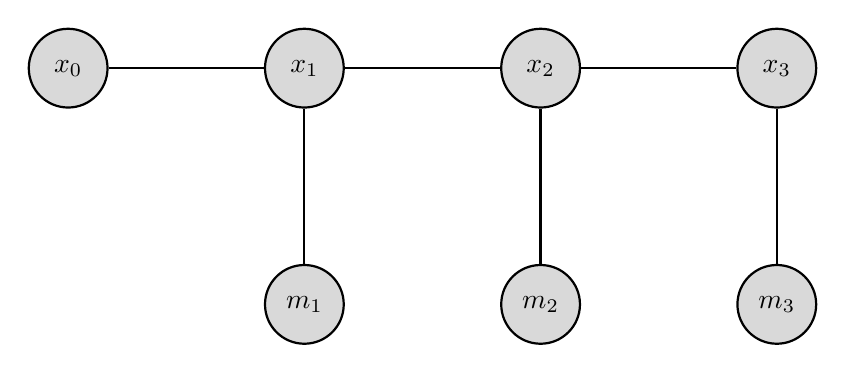
\begin{tikzpicture}[scale=1, thick]
        % states
        \node (x0) at (0,0) [shape=circle,draw=black, fill=gray!30, minimum size=1cm] {$x_0$};
        \node (x1) at (3,0) [shape=circle,draw=black, fill=gray!30, minimum size=1cm] {$x_1$};
        \node (x2) at (6,0) [shape=circle,draw=black, fill=gray!30, minimum size=1cm] {$x_2$};
        \node (x3) at (9,0) [shape=circle,draw=black, fill=gray!30, minimum size=1cm] {$x_3$};

        % landmarks
        \node (m1) at (3,-3) [shape=circle,draw=black, fill=gray!30, minimum size=1cm] {$m_1$};
        \node (m2) at (6,-3) [shape=circle,draw=black, fill=gray!30, minimum size=1cm] {$m_2$};
        \node (m3) at (9,-3) [shape=circle,draw=black, fill=gray!30, minimum size=1cm] {$m_3$};

        % connections
        \draw[-] (x0) -- (x1);
        \draw[-] (x1) -- (x2);
        \draw[-] (x2) -- (x3);
        \draw[-] (m1) -- (x1);
        \draw[-] (m2) -- (x2);
        \draw[-] (m3) -- (x3);

        % observed
        % \node (x0) at (-2,-2) [shape=circle,draw=black, fill=gray!70, minimum size=1cm] {$x_0$};



        % \node (x1) at (-0.66,-2) [shape=circle,draw=black, fill=gray!70, minimum size=1cm] {$x_1$};
        % \node (dots) at (0.66,-2) {\ldots};
        % \node (xn) at (2,-2) [shape=circle,draw=black, fill=gray!70, minimum size=1cm] {$x_N$};
        % \draw[->] (z) -- (x0);
        % \draw[->] (z) -- (x1);
        % \draw[->] (z) -- (xn);
    \end{tikzpicture}
\end{document}